\documentclass[tikz]{standalone}
% \documentclass{article}
\usepackage{tikz}
\usepackage{amsmath}
\usepackage{mathtools}
% \usepackage{decorate}

\begin{document}
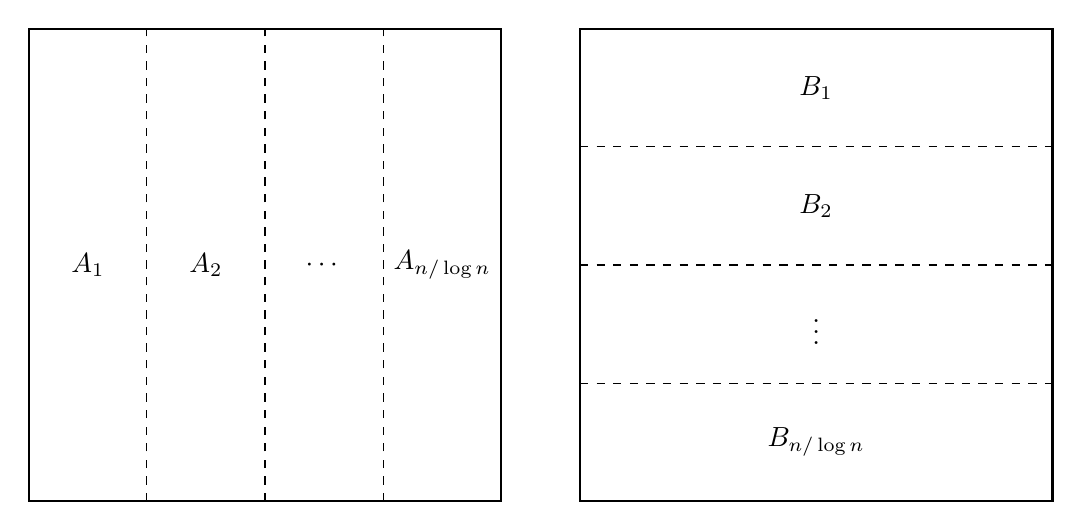
\begin{tikzpicture}[scale=1, every node/.style={scale=1}]

% Dimensions
\def\width{6}
\def\height{6}
\def\nparts{4}

% A matrix - vertical divisions
\draw[thick] (0, 0) rectangle (\width, \height);
\foreach \i in {1,...,4} {
    \draw[dashed] ({\width/\nparts * \i}, 0) -- ({\width/\nparts * \i}, \height);
}

% B matrix - horizontal divisions
\draw[thick] (\width + 1, 0) rectangle (\width*2 + 1, \height);
\foreach \i in {1,...,4} {
    \draw[dashed] (\width + 1, {\height/\nparts * \i}) -- (\width*2 + 1, {\height/\nparts * \i});
}

% Labels A_i
\node at ({\width/\nparts * 0.5}, \height/2) {$A_1$};
\node at ({\width/\nparts * 1.5}, \height/2) {$A_2$};
\node at ({\width/\nparts * 2.5}, \height/2) {$\cdots$};
\node at ({\width/\nparts * 3.5}, \height/2) {$A_{n / \log n}$};

% Labels B_i
\node at (1 + 1.5*\width, {\height/\nparts * 3.5}) {$B_1$};
\node at (1 + 1.5*\width, {\height/\nparts * 2.5}) {$B_2$};
\node at (1 + 1.5*\width, {\height/\nparts * 1.5}) {$\vdots$};
\node at (1 + 1.5*\width, {\height/\nparts * 0.5}) {$B_{n / \log n}$};

\end{tikzpicture}
\end{document}
